%\note{Все живые организмы дышат, т. е. поглощают кислород и выделяют углекислый газ и воду. При этом происходит разложение органических веществ и выделение энергии, необходимой для жизни каждой клетки, всего растения.}

\subsection*{Общие сведения о процессе дыхания}

%Процесс превращения исходного органического вещества до более простых и затем до СО2 и Н2О требует большого числа различных ферментов.

\subsubsection*{Суммарное уравнение дыхания}

\begin{equation}
	 C_{6}H_{12}O_{6} + 6O_{2} = 6CO_{2} + 6H_{2}O.
	 \label{braezing_balance}
\end{equation}

\note{Данная формула характеризует начальный и конечный момент процесса \hypertarget{sect_breazing}{дыхания}. В действительности этот процесс многоступенчатый. Он состоит из целого ряда последовательно идущих окислительно-восстановительных реакций.}

%Итак, для дыхания нужно органическое вещество, включающее в себя запас потенциальной энергии, и кислород.

\subsubsection*{Субстраты дыхания}

\paragraph*{}В процессе дыхания окислению могут подвергаться большое количество разнообразных органических веществ, чаще всего это:

\begin{enumerate}

\item углеводы
\item белки 
\item жиры. 

\end{enumerate}

\paragraph*{}Типичным и наиболее выгодным для дыхания соединением, окисляемым в процессе дыхания, является глюкоза.  

\paragraph*{}По отношению объемов поглощенного организмом кислорода и выделенного углекислого газа, можно сделать вывод о химической природе используемого в процессе дыхания. Так, при окислении глюкозы, как следует из балансового уравнения \ref{braezing_balance} объемы выделенного при дыхании углекислого газа и поглощенного кислорода, должны быть равны. 

\remember{Отношение объема выделившегося углекислого газа к объему поглощенного кислорода $CO_{2}/O_{2}$ называется \hypertarget{breazing_index}{\gls{breazingIndex}}}

\paragraph*{}Если исходным дыхательным материалом является сахар, то этот коэффициент обычно равен 1.

\paragraph*{}В том случае, когда исходным материалом будут жиры или белки, на окисление которых нужно больше кислорода из воздуха, дыхательный коэффициент снизится до 0,7-0,8.

\note{Например, если исходным веществом будет стеариновая кислота, то процесс дыхания пойдет по суммарному уравнению:



$C_{18}H_{36}O_{2} + 26O_{2}  = 18CO_{2} + 18H_{2}O$



В данном случае, дыхательный коэффициент будет равен 18:26 = 0,69.}

\paragraph*{}Если же исходным веществом будут соединения, богатые кислородом, то для их окисления потребуется меньше кислорода воздуха, и дыхательный коэффициент повысится.

\note{Так, при дыхании за счет щавелевой кислоты уравнение примет следующий вид:



$2C_{2}O_{4}H_{2} + O_{2} = 4CO_{2} + 2H_{2}O$



Дыхательный коэффициент будет равен 4/1 = 4. }

\paragraph*{}Чем выше дыхательный коэффициент, тем ниже тепловой эффект, и наоборот. Поэтому жиры и белки отличаются более высоким тепловым эквивалентом.
%Сравнивать дыхание у разных органов растения можно по выделению СО2 на 1 г сухого вещества в единицу времени при определенной температуре, т. е. по интенсивности дыхательного процесса.

\paragraph*{}Определению дыхательного коэффициента прорастающих семян посвящена одна из \hyperlink{breazing_index_lab}{лабораторных работ}.

\note{Установлено, что растущие органы дышат интенсивнее нерастущих. Прорастающие семена, цветки, плоды, мицелий грибов дышат более интенсивно, чем другие органы.} 

\paragraph*{}Фотосинтез и дыхание можно рассматривать как два противоположных процесса. Если в растении оба процесса будут протекать с одинаковой интенсивностью, то накопления органического вещества не будет. В пасмурную и холодную погоду такое явление может произойти. 

\paragraph*{}Интенсивность света, при которой количество создаваемого органического вещества при фотосинтезе равно трате его на дыхание, называется компенсационной точкой. Для световых и теневых растений компенсационная точка будет различная.

\subsection*{Факторы, влияющие на интенсивность дыхания}

\paragraph*{}На интенсивность дыхания влияют следующие факторы

\begin{enumerate}

\item температура, 
\item влажность, 
\item наличие ядовитых веществ и физических агентов, 
\item содержание кислорода в воздухе.

\end{enumerate}

\subsubsection*{Влияние температуры воздуха и почвы}


\paragraph*{}Влияние температуры на жизненные процессы подчиняется правилу Вант-Гоффа, согласно которому, при повышении температуры на каждые 10 \celsius скорость процесса удваивается. Это ускорение носит название температурного коэффициента. Он равен примерно 2. \gls{VanGoffRule} действует в \hyperlink{question_van_goff}{пределах} до 40 \celsius. 

\paragraph*{}Дыхание у растений происходит в довольно широких границах температур.

\note{У зимующих растений дыхание можно обнаружить и при 20-25 \celsius мороза}

\paragraph*{}Оптимальная температура для дыхания прорастающих семян 30 и 40 \celsius. При температуре 50 \celsius дыхание прекращается, так как белки цитоплазмы свертываются.

\subsubsection*{Насыщенность клеток водой}

\paragraph*{}Вода необходима для набухания коллоидов цитоплазмы. 
Сухие семяна выделят очень незначительное количество углекислого газ. Во влажных семенах выделение $CO_{2}$ увеличивается в 10000 раз. Поэтому хранение зерна, имеющего влажность свыше 12-14 \%, приводит к потере органического вещества и всхожести. 
Зерно темнеет и портится (<<сгорает>>).

\note{Например, семена ячменя (с 10-12 \% гигроскопической воды) выделяют за сутки ничтожное количество углекислого газа (0,3-0,4 мг). При повышении содержания воды до 33 \% (почти полном набухании) количество выделенного $CO_{2}$ достигает 2 г)}

\subsubsection*{Наличие ядовитых веществ и физических агентов}

\paragraph*{}Такие вещества, как 

\begin{enumerate}

\item эфир
\item хлороформ 
\item нейтральные соли щелочных и щелочно-земельных металлов

\end{enumerate}
 
в больших дозах вызывают быстрое падение дыхания вследствие отравления растения. В малых дозах они действуют стимулирующее -- интенсивность дыхание повышается.

\subsubsection*{Влияние концентрации кислорода в воздухе}

\paragraph*{}Небольшие колебания в содержании кислорода в воздухе (20,95 \%) особого влияния на процесс дыхания не оказывают. Падение же его содержания до 1-2 \% приводит обычно к снижению интенсивности дыхания. 

\note{Недостаток кислорода возможен и внутри некоторых семян, имеющих плотную кожуру. Накопившийся в них углекислый газ действует на семена как анестезирующее средство (делающее их нечувствительными). Не теряя всхожести, такие семена могут длительное время находиться в почве, не прорастая (многие сорняки). В настоящее время $CO_{2}$ применяют для сохранения плодов и овощей.}

%Дыхание и брожение в современном изложении

%Процессы дыхания и брожения имеют очень сложные срединные звенья, связанные с образованием многих промежуточных продуктов. Благодаря этому указанные процессы тесно связаны с общим обменом веществ в растении.
%В результате более детального исследования спиртового брожения было выяснено, что оно является по существу первой фазой дыхания. Лишь вторая фаза, после образования пировиноградной кислоты, будет у обоих процессов различна. 
 
%Далее при дыхании происходит ступенчатое превращение последней в присутствии кислорода в СО2 и Н2О с выделением (в целом) 686 ккал энергии. Оно называется циклом Кребса. 

\subsection*{Гликолиз}

%При брожении пировиноградная кислота в отсутствие кислорода постепенно превращается в спирт и СО2 с выделением 24 ккал.

\termin{\hypertarget{glycolysis}{\gls{glycolisys}}} -- это процесс распада сахаров, который происходит с образованием глюкоза-6-фосфата и заканчивается образованием прировиноградной кислоты.

\paragraph*{}Гликолиз является первой стадией как брожения так и аэробного дыхания.

\paragraph*{}Реакции гликолиза происходят в \hyperlink{protoplast}{цитоплазме} и в \hyperlink{plastides}{хлоропластах}. Последовательность реакций гликолиза можно разделить на три стадии:

\begin{enumerate}
	\item Подготовительный этап. В ходе данного этапа образуется фруктозо-1,6-бисфосфат, который затем расщепляется на две фосфотриозы: \gls{fgal} и \termin{фосфодиоксиацетон}.
	\item Первое \hypertarget{substratickFosforolysis}{субстратное фосфорилирование}. На этом этапе \gls{fgal} сначала окисляется с образованием \gls{nadh} и 1,3-бисфосфоглицериновой кислоты (1,3-\gls{fgac}). Затем 1,3-\gls{fgac} дефосфорилируется с образованием \gls{atp} и 3-\gls{fgac}.
	\item Второе субстратное фосфорилирование, В ходе этого этапа происходит образование еще одной молекулы \gls{atp} при переносе фосфатной группы с фосфоенолпировиноградной кислоты \gls{fep} на АДФ.

\end{enumerate}

%АТФ в растении образуется не только в хлоропластах, о чем было сказано ранее, но и в митохондриях, при наличии кислорода и окислительных ферментов. Такой способ образования АТФ называется окислительным фосфорилированием (в отличие от фотосинтетического фосфорилирования). Энергию для реакции АДФ + Н3РО4 = АТФ + Н2О растение получает в результате процесса дыхания, а не солнца. При переходе АТФ – АДФ растение получает 8— 10 ккал, которые используются для эндотермических (требующих затраты энергии) реакций.
%Чтобы яснее представить сложность гликолиза, рассмотрим ход последовательных превращений глюкозы до \gls{pva}:

\paragraph*{}Обобщив вышесказанное, можно составить следующую цепь превращений, происходящих в ходе \gls{glycolisys}а:

Глюкоза $\rightarrow$ Глюкозо-6-фосфат $\rightarrow$ Фруктозо-1,6-дифосфат $\rightarrow$ \gls{fgal} $\rightarrow$ Дифосфоглицериновая кислота $\rightarrow$ 3-\gls{fgac} $\rightarrow$ 2-Фосфоглицериновая кислота $\rightarrow$ Фосфоэнолпировиноградная кислота $\rightarrow$ Энолпировиноградная кислота $\rightarrow$ \gls{pva}.

\subsubsection*{Энергетика гликолиза}

\paragraph*{}На образование фруктоза-1,6-бифосфата тратится 2 молекулы \gls{atp}. В результате же двух субстратных фосфорелирований образуется 4 молекулы \gls{atp}. Таким образом, <<чистый>> энергетический выход гликолиза -- 2 молекулы \gls{atp} (4-2=2). Кроме того, в результате гликолиза образуется 2 молекулы \gls{nadh}. 

\paragraph*{}Учитывая то, что в аэробных условиях окисление \gls{nadh} приведет к образованию еще 6-и молекул \gls{atp}, энергетический выход гликолиза в аэробных условиях будет 8 молекул \gls{atp} (2+6=8).

\paragraph*{}В дальнейшем, образовавшаяся пировиноградная кислота в процессе дыхания претерпевает превращения в ходе реакций цикла Кребса.

\subsubsection*{Отличительные особенности гликолиза в клетках растений}

\paragraph*{}В отличии от клеток животных, процесс \gls{glycolisys}а в растительной клетке имеет следующие особенности \cite{medvedev_2012}:

\begin{enumerate}

\item У растений \gls{glycolisys} может идти не только в цитоплазме, но и в хлоропластах
\item В отличии от животных, исходным соединением для гликолиза является не глюкоза а сахароза.
\item Конечным продуктом гликолиза может быть не только \gls{pva}, но и малат

\end{enumerate}

\subsection*{Цикл Кребса}  

\paragraph*{}\hypertarget{krebs_cycle}{Цикл Кребса}\footnote{Нередко цикл Кребса называют лимонно-кислым циклом или циклом трикарбоновых кислот}, является основным этапом процесса дыхания. Этот процесс практически универсален, является главным путем окисления остатков уксусной кислоты у всех живых организмов. Цикл Кребса происходит в матриксе \hyperlink{митохондрий}.     
  
%В ходе видоизменения одних кислот в другие выделяются СО2 и Н2О. Углерод окисляется кислородом воды, а не кислородом из внешней среды. Последний же окисляет выделяющийся водород и образует воду.


\paragraph*{}Цикл Кребса (\ris \ref{krebs_cycle}) включает в себя 8 последовательных реакций и состоит из двух стадий.

%%%%%%%%%%%%%%%%%%%%%%%%%%%%%%%%%%%%%%%%%%%%%%%%%%%%%%%%%%%%%%%%%%%%%%%%%%%%%%%%%%%%%%%%%%%%%%%%%%%%%%%%%%% 
\begin{figure}
  \centering
       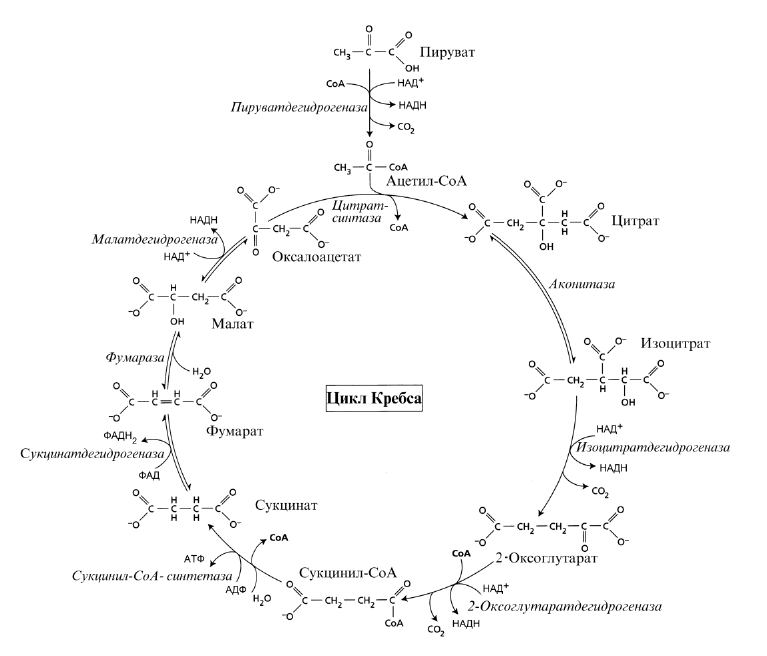
\includegraphics[width=1\linewidth]{pictures/krebs_cycle}
\caption{Схема реакций цикла Кребса}
\paragraph*{}Приведена из \cite{medvedev_2012}
\label{krebs_cycle}
\end{figure}
%%%%%%%%%%%%%%%%%%%%%%%%%%%%%%%%%%%%%%%%%%%%%%%%%%%%%%%%%%%%%%%%%%%%%%%%%%%%%%%%%%%%%%%%%% 

\begin{enumerate}

\item В начале цикла от молекулы \gls{pva} отделяется одна молекула углекислого газа, а оставшийся фрагмент, в виде ацетильного остатка соединяется с коэнзимом А. Отщепление углекислого газа от пировиноградной кислоты носит название \termin{декарбоксилирование}. Образовавшийся при этом \gls{acetylCoensimA},является ключевым веществом, входящим в собственно цикл Кребса\footnote{\gls{acetylCoensimA} может образовываться и в результате ряда других химических реакций}

\item \gls{acetylCoensimA} включается в цикл Кребса путем присоединения его к щавелевоуксусной кислоте (четырехуглеродному соединению, дикарбоновой кислоте), в результате чего образуется лимонная кислота (шестиуглеродное соединение, трикарбоновая кислота). После образования лимонной кислоты через ряд промежуточных соединений происходит образование 
щавелевоуксусной кислоты, при этом выделяется две молекулы $CO_{2}$ и 8$H^{+}$.

\end{enumerate}

\paragraph*{}Ниже перечислена последовательность реакций цикла Кребса и \hyperlink{enzimes}{ферменты} участвующие в этих реакциях:

\begin{enumerate}

\item Aцетильная группа \gls{acetylCoensimA} конденсируется с оксалоацетатом, в результате чего образуется лимонная кислота. Реакция катализируется \termin{цитрат-синтазой}

\item Лимонная кислота подвергается дегидратированию с образованием \termin{цис-аконитовой кислоты}, затем, к цис-аконитовой кислоте присоединяется молекула воды. При этом цис-аконитовая ксилота переходит в изолимонную кислоту (изоцитрат). Катализирует эти обратимые реакции фермент \termin{аконитатгидратаза}. В результате происходит взаимоперемещение Н и ОН в молекуле цитрата:

\item Изолимонная кислота дегидрируется при участии фермента \termin{НАД-зависимой изо-цитратдегидрогеназы.}

\item В результате окислительного декарбоксилирования $\alpha$-кетоглутаровой кислоты образуется высокоэнергетическое соединение сукцинил-КоА. В данной реакции принимают участие 5 \gls{coenzim}ов: ТПФ, амид липоевой кислоты, HS-KoA, ФАД и НАД+.

\item Сукцинат дегидрируется в фумаровую кислоту. Окисление сукцината катализируется сукцинатдегидрогеназой, в молекуле которой с белком прочно (ковалентно) связан \gls{coenzim} ФАД. \note{В свою очередь сукцинатдегидрогеназа прочно связана с внутренней ми-тохондриальной мембраной}

\item Фумаровая кислота гидратируется, продуктом реакции является яблочная кислота (малат). Реакция осуществляется под влиянием фермента \termin{фумаратгидратазы} (фумаразы).

\item Под влиянием митохондриальной НАД-зависимой малатдегидрогеназы происходит окисление L-малата в оксалоацетат

\end{enumerate}

\paragraph*{}Через образование \gls{pva} и ряда других органических кислот в процесс дыхания поступают также продукты разложения белков -- аминокислоты. При этом углеродные скелеты аминокислот подвергаются окислительному расщеплению на фрагменты. 

\note{Такие аминокислоты как аланин, цистеин, глицин, серин и треонин образуют \gls{acetylCoensimA} через пировиноградную кислоту, а лейцин, лизин, фенилаланин, тирозин и триптофан образуют \gls{acetylCoensimA} через ацетоацетилКоА. Пролин, гистидин, аргинин, глутамин и клутаминовая кислота включаются в цикл Кребса через a-кетоглутаровую кислоту, метионин, изолейцин и валин - через янтарную кислоту, фенилаланин и тирозин - через фумаровую кислоту, аспарагин и аспарагиновая кислота - через щавелевоуксусную кислоту.}

\remember{Физиологический смысл цикла Кребса состоит в том, что именно здесь происходит разложение органического вещества (\gls{pva}) до неорганических веществ (углекислого газа и ионов водорода), при этом образуется большое количество энергии в виде молекул \gls{atp}.}

\subsubsection*{Энергетика цикла Кребса}

\paragraph*{}Таким образом, одна молекула \gls{nadh} образуется при окислительном декарбоксилировании пирувата в\gls{acetylCoensimA}. При участии данной молекулы позже образуются 3 молекулы \gls{atp} 

\paragraph*{}При расщеплении одной молекулы глюкозы образуется 2 молекулы пировиноградной кислоты, а при окислении их до 2 молекул \gls{acetylCoensimA} и последующих 2 оборотов цикла Кребса синтезируется еще 30 молекул \gls{atp}. 

\paragraph*{}Если учесть, что 8 молекул \gls{atp}, образующихся при аэробном \hyperlink{glycolysis}{гликолизе}, то, суммарно, при расщеплении в тканях одной молекулы глюкозы по уравнению \ref{braezing_balance} синтезируется 38 молекул \gls{atp}. 



\subsubsection*{Значение цикла Кребса}

\begin{enumerate}

\item \gls{acetylCoensimA} служит исходным продуктом для синтеза жирных кислот, для некоторых гормонов, терпенов, изопреноидов и стероидов.
\item Промежуточные продукты цикла Кребса являются <<сырьем>> для синтеза аминокислот, которые могут быть использованы растением в обмене веществ. Так некоторые кислоты (фумаровая, яблочная и др.), при присоединении к ним аминогруппы преобразуются в аминокислоты. Важную роль в этом процессе играют реакции трансаминирования, при этом аминогруппы большинства аминокислот переносятся на пировиноградную, щавелевоуксусную или a-кетоглутаровую кислоты.

\end{enumerate}

\subsection*{Гликооксалатный путь}

\subsection*{Вопросы и задания для самоконтроля}

\begin{enumerate}

\item В чем состоит значение процесса дыхания в \gls{metabolism}е клетки? 
\item Каково суммарное уравнение реакций аэробного дыхания? 
\item Повторите особенности организации белковой молекулы. Почему, на ваш взгляд, интенсивность дыхания резко \hypertarget{question_van_goff}{падает} при температуре выше 50 \celsius.
\item Что такое окислительное фосфорилирование? 
\item В чем заключается роль гликолиза в \gls{metabolism}е клетки? 
\item Какие вещества поступают в цикл Кребса а какие выходят из него?
\item В чем заключается значение цикла Кребса для \gls{metabolism}а клетки?
\item В чем заключается сходство и различие между анаэробным дыханием в растительной клетки и спиртовым брожением?
\item Как происходят масляно-кислое и молочно-кислое брожения? У каких организмов происходит брожение такого типа?

\end{enumerate}
